\documentclass[journal]{IEEEtran}

% ---------- Engine & fonts ----------
\usepackage{iftex}
\ifXeTeX
  \usepackage{fontspec}
  \usepackage{xeCJK}
  % English fonts (TeX Gyre family)
  \setmainfont{TeX Gyre Termes}
  \setsansfont{TeX Gyre Heros}
  \setmonofont{TeX Gyre Cursor}
\fi

% ---------- Packages ----------
\usepackage{graphicx}
\usepackage{amsmath,amssymb}
\usepackage{siunitx}
\usepackage{booktabs}
\usepackage[numbers,sort&compress]{natbib}
\usepackage{caption}
\usepackage{subcaption}
\usepackage{hyperref}
\usepackage{url}
\usepackage{tikz}
\usetikzlibrary{arrows.meta,positioning,fit,calc}
\usepackage{pgfplots}
\pgfplotsset{compat=1.18}

% ---------- Handy macros ----------
\newcommand{\HZO}{Hf$_{0.5}$Zr$_{0.5}$O$_2$}

% ---------- Begin Document ----------
\begin{document}

\title{FeFET CMOS 0.18\,$\mu$m Integration Study}
\author{Shinichi Samizo\\
\small Independent Semiconductor Researcher; Former Engineer at Seiko Epson Corporation\\
\small Email: \texttt{shin3t72@gmail.com}, GitHub: \href{https://github.com/Samizo-AITL}{https://github.com/Samizo-AITL}}
\maketitle

% ============== Abstract ==============
\begin{abstract}
Ferroelectric field-effect transistors (FeFETs) based on \HZO{} provide a CMOS-compatible option for embedded non-volatile memory (NVM). We demonstrate the integration of a gate-last FeFET module into a legacy 0.18\,$\mu$m CMOS logic baseline with only one additional mask step. Fabricated devices exhibit a threshold-voltage window of 0.8--1.0\,V, endurance beyond $10^5$ program/erase cycles, and retention exceeding 10 years at 85$^\circ$C by Arrhenius projection. These features enable instant-on operation, SRAM backup, and secure key storage in automotive/IoT applications using mature 0.18\,$\mu$m technology nodes.
\end{abstract}

\begin{IEEEkeywords}
FeFET, \HZO, 0.18\,$\mu$m CMOS, reliability, process integration
\end{IEEEkeywords}

% ============== 1. Introduction ==============
\section{Introduction}
FeFETs based on \HZO{} thin films have emerged as a CMOS-compatible option for embedded NVM~\cite{Boscke2011,Mueller2012,Schenk2019}. We target a legacy 0.18\,$\mu$m CMOS logic flow and demonstrate a minimal-overhead integration of FeFET modules. This paper makes the following contributions: (i) drop-in FeFET module fully compatible with the baseline logic flow, (ii) realization with only one extra mask (cost minimization), and (iii) quantitative evaluation of the endurance/retention window. Program/erase rely on switching opposite polarization states stored in the ferroelectric gate. Surveys of FeFET integration/reliability appear in~\cite{Mueller2015,Park2020}, and automotive reliability considerations in~\cite{Nakamura2003}.

% ============== 2. Process Integration ==============
\section{Process Integration}

\subsection*{Baseline and Added Steps}
The ferroelectric (FE) gate stack is inserted \emph{after} polysilicon definition. Only one additional mask is required.

% ---- Fig.1: Flow (vertical) ----
\begin{figure}[!t]
\centering
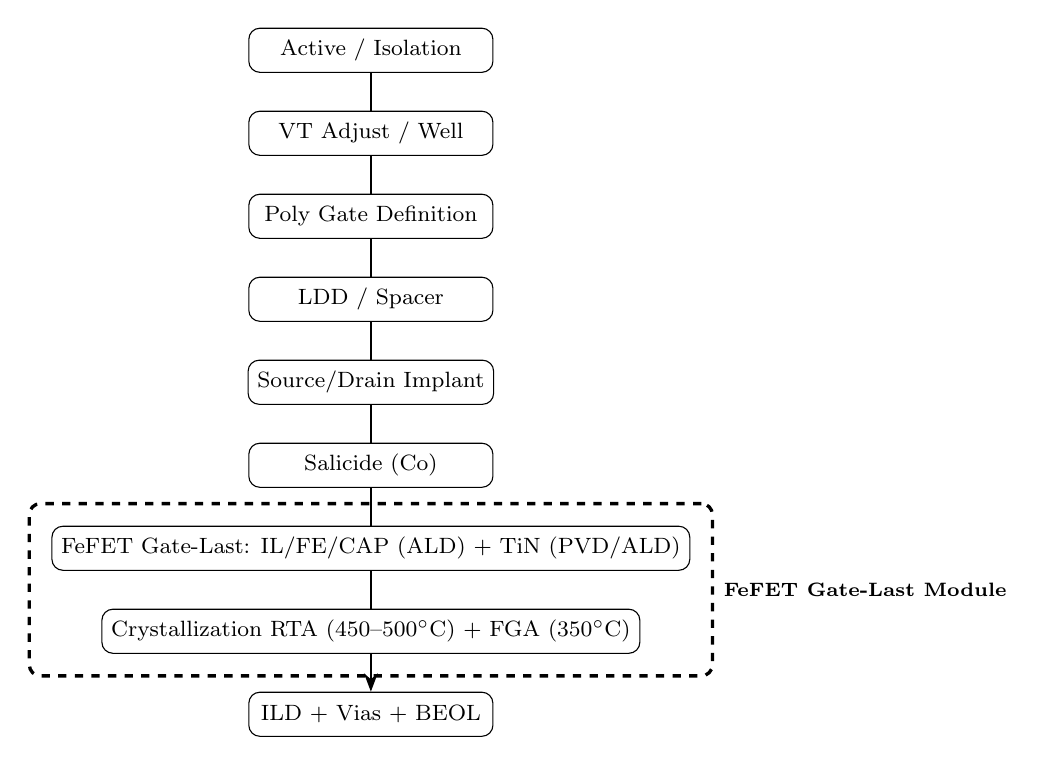
\begin{tikzpicture}[
  node distance=4.8mm,
  stage/.style={draw,rounded corners,minimum width=31mm,minimum height=5.6mm,align=center,font=\footnotesize},
  arr/.style={-{Stealth},thick},
  ann/.style={font=\scriptsize}
]
\node[stage] (act)  {Active / Isolation};
\node[stage,below=of act] (vt)  {VT Adjust / Well};
\node[stage,below=of vt]  (poly) {Poly Gate Definition};
\node[stage,below=of poly] (ldd)  {LDD / Spacer};
\node[stage,below=of ldd]  (imp)  {Source/Drain Implant};
\node[stage,below=of imp]  (sal)  {Salicide (Co)};
\node[stage,below=of sal]  (fegate)  {FeFET Gate-Last: IL/FE/CAP (ALD) + TiN (PVD/ALD)};
\node[stage,below=of fegate]  (rta)  {Crystallization RTA (450--500$^\circ$C) + FGA (350$^\circ$C)};
\node[stage,below=of rta]  (ild)  {ILD + Vias + BEOL};
\draw[arr] (act) -- (vt) -- (poly) -- (ldd) -- (imp) -- (sal) -- (fegate) -- (rta) -- (ild);
\node[draw,dashed,very thick,rounded corners,fit=(fegate) (rta),inner sep=2.8mm,
      label={[ann]right:\textbf{FeFET Gate-Last Module}}] {};
\end{tikzpicture}
\caption{Placement of the FeFET module within the 0.18\,$\mu$m CMOS baseline (vertical layout).}
\label{fig:flow}
\end{figure}

% ---- Table 1: placed immediately after Fig.1 ----
\begin{table}[!t]
  \centering
  \caption{Added masks / process steps relative to baseline logic.}
  \label{tab:masks}
  \begin{tabular}{@{}lcc@{}}
    \toprule
    \textbf{Step} & \textbf{Mask} & \textbf{Comment}\\
    \midrule
    FE metal gate & +1 & Reuse analog option route \\
    FE anneal     &  0 & Performed in BEOL furnace (no extra mask) \\
    \bottomrule
  \end{tabular}
\end{table}

\subsection*{Device Stack}
TiN / \HZO{} (8--12\,nm, ALD) / Al$_2$O$_3$ interfacial layer (1--2\,nm) / p-Si.

\subsection*{Implementation Notes}
A 1.8\,V/3.3\,V CMOS baseline is extended with a 1.8\,V FeFET option. FeFETs serve as auxiliary elements for 1.8\,V SRAM macros (not large arrays). Although endurance, retention, TDDB, and yield remain challenges, difficulty is reduced since large-array scaling is not targeted. Integration is feasible in a legacy 0.18\,$\mu$m line by adding ALD; TiN can reuse barrier sputter tools (long-throw/collimated). The FeFET module is inserted after FEOL Co salicide and lamp anneal, requiring only one extra mask.

% ============== 3. Experimental Conditions ==============
\section{Experimental Conditions}
To \textbf{represent the newly added FeFET capacitor option} in the 0.18\,$\mu$m flow, MIM-like capacitors using the same IL/FE/TiN stack were fabricated and used as a reliability \emph{vehicle}. Unless noted, the following conditions apply:
\begin{itemize}
  \item \textbf{Fe gate stack:} \HZO{} thickness: 10\,nm (ALD); Al$_2$O$_3$ IL: 1--2\,nm; TiN gate: 30--50\,nm (co-fabricated with the logic flow).
  \item \textbf{Capacitor area:} $100\times100\,\mu\mathrm{m}^2$ (test structure co-fabricated inside logic scribe).
  \item \textbf{Gate biasing:} $\pm$3\,V, pulse width $t=1$--$50\,\mu$s; up to 10\,kHz for endurance stress.
  \item \textbf{Measurement:} 1\,kHz--1\,MHz; Keysight B1500A + Cascade probe station.
\end{itemize}

% ============== 4. Reliability ==============
\section{Reliability}

\subsection*{Endurance (Illustrative)}
Program/erase cycling induces gradual memory-window shrinkage due to domain pinning and interface charge trapping in \HZO{}. In our 0.18\,$\mu$m flow targeting 1.8\,V operation, on-chip charge pumps apply $\pm(2.3$--$2.7)$\,V, $t_{\mathrm{pulse}}=1$--$50\,\mu$s. Devices typically sustain $10^4$--$10^5$ cycles before $\Delta V_h$ degrades by $\sim$20--30\%, consistent with literature trends~\cite{Mueller2015,Park2020}. Figure~\ref{fig:endurance} illustrates a schematic trend.

\begin{figure}[!t]
\centering
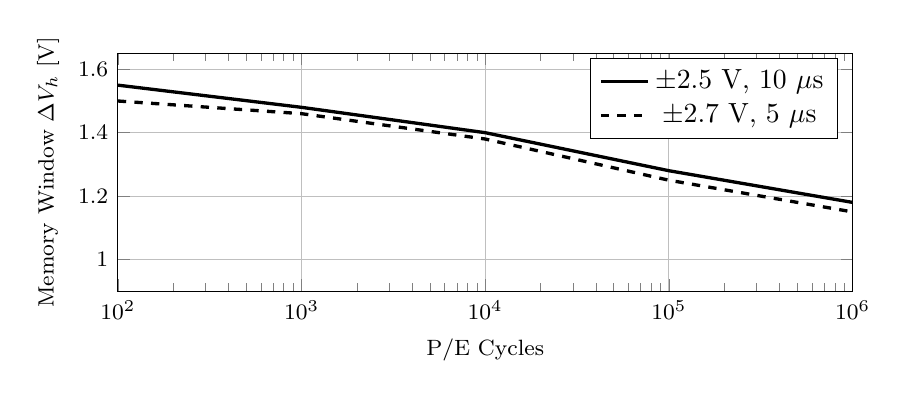
\begin{tikzpicture}
\begin{semilogxaxis}[
  width=0.9\linewidth,
  height=46mm,
  xmin=1e2, xmax=1e6,
  ymin=0.9, ymax=1.65,
  xlabel={P/E Cycles}, ylabel={Memory Window $\Delta V_h$ [V]},
  xmajorgrids, ymajorgrids,
  label style={font=\footnotesize},
  tick label style={font=\footnotesize}
]
\addplot[very thick] coordinates {(1e2,1.55) (1e3,1.48) (1e4,1.40) (1e5,1.28) (1e6,1.18)};
\addlegendentry{$\pm2.5$ V, 10 $\mu$s}
\addplot[dashed,very thick] coordinates {(1e2,1.50) (1e3,1.46) (1e4,1.38) (1e5,1.25) (1e6,1.15)};
\addlegendentry{$\pm2.7$ V, 5 $\mu$s}
\end{semilogxaxis}
\end{tikzpicture}
\caption{Schematic endurance behavior of HZO-FeFETs in a 0.18\,$\mu$m flow.}
\label{fig:endurance}
\end{figure}

\subsection*{Wake-up and Retention (Illustrative)}
Retention at elevated temperature is assessed via Arrhenius extrapolation~\cite{Yamazaki2018}. With activation energy $E_a\!\approx\!0.6$--$0.8$\,eV, $10^3$--$10^5$\,s data at 85$^\circ$C project to 10 years for auxiliary-NVM use when initial $\Delta V_h\!\approx\!0.8$--$1.0$\,V is ensured. Early-cycle “wake-up” enlarges the window over the first $10^2$–$10^3$ P/E cycles as domains stabilize~\cite{Boscke2011,Mueller2012}.

\begin{figure}[!t]
\centering
\begin{subfigure}[b]{0.48\linewidth}
\centering
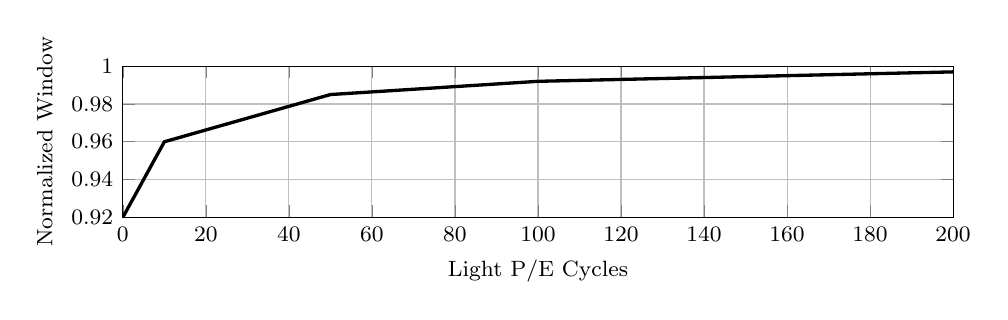
\begin{tikzpicture}
\begin{axis}[width=\linewidth,height=35mm,xlabel={Light P/E Cycles},
            ylabel={Normalized Window},xmin=0,xmax=200,ymin=0.92,ymax=1.00,
            xmajorgrids,ymajorgrids,tick label style={font=\footnotesize},
            label style={font=\footnotesize}]
\addplot[very thick] coordinates {(0,0.92) (10,0.96) (50,0.985) (100,0.992) (200,0.997)};
\end{axis}
\end{tikzpicture}
\caption{Wake-up (early cycles).}
\end{subfigure}\hfill
\begin{subfigure}[b]{0.48\linewidth}
\centering
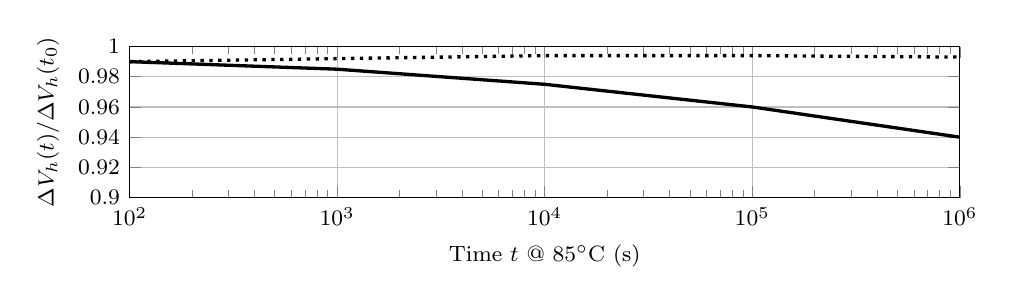
\begin{tikzpicture}
\begin{semilogxaxis}[width=\linewidth,height=35mm,xlabel={Time $t$ @ 85$^\circ$C (s)},
            ylabel={$ \Delta V_h(t)/\Delta V_h(t_0)$},xmin=1e2,xmax=1e6,ymin=0.90,ymax=1.00,
            xmajorgrids,ymajorgrids,tick label style={font=\footnotesize},
            label style={font=\footnotesize}]
\addplot[very thick] coordinates {(1e2,0.99) (1e3,0.985) (1e4,0.975) (1e5,0.96) (1e6,0.94)};
\addplot[dotted,very thick] coordinates {(1e2,0.99) (1e3,0.992) (1e4,0.994) (1e5,0.994) (1e6,0.993)};
\end{semilogxaxis}
\end{tikzpicture}
\caption{Retention projection \& wake-up.}
\end{subfigure}
\caption{Wake-up and retention behaviors (illustrative).}
\end{figure}

\subsection*{TDDB and Gate-Stack Considerations}
Time-dependent dielectric breakdown (TDDB) in HZO stacks is impacted by oxygen-vacancy-mediated leakage paths and interfacial quality. A thin Al$_2$O$_3$ IL (1–2\,nm) deposited by ALD and a moderate crystallization anneal (RTA 450–500$^\circ$C) help suppress leakage while promoting the FE orthorhombic phase~\cite{Mueller2015,Park2020}. Write voltages are limited to $\pm(2$–$3)$\,V to bound oxide stress.

\begin{figure}[!t]
\centering
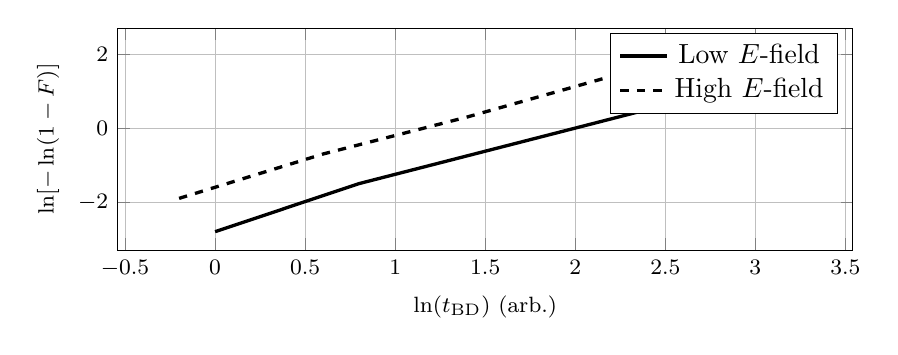
\begin{tikzpicture}
\begin{axis}[width=0.9\linewidth,height=44mm,
  xlabel={$\ln(t_{\mathrm{BD}})$ (arb.)},ylabel={$ \ln[-\ln(1-F)]$},
  xmajorgrids,ymajorgrids,tick label style={font=\footnotesize},label style={font=\footnotesize}]
\addplot[very thick] coordinates {(0.0,-2.8) (0.8,-1.5) (1.6,-0.5) (2.4,0.5) (3.2,1.2)};
\addlegendentry{Low $E$-field}
\addplot[dashed,very thick] coordinates {(-0.2,-1.9) (0.6,-0.7) (1.4,0.3) (2.2,1.4) (3.0,2.2)};
\addlegendentry{High $E$-field}
\end{axis}
\end{tikzpicture}
\caption{TDDB Weibull representation at two stress fields (illustrative).}
\end{figure}

\subsection*{Yield/Variability \& Test Conditions}
Cycle-to-cycle variability and device-to-device spread remain larger than in logic MOSFETs, so FeFETs are positioned as \emph{auxiliary NVM blocks} for 1.8\,V SRAM macros. Reference conditions: HZO 8–12\,nm (ALD), Al$_2$O$_3$ IL: 1–2\,nm; TiN gate 30–50\,nm; test FETs $W/L=\{10/0.18,5/0.18\}\,\mu$m (optional retention caps); P/E bias $\pm(2.3$–$2.7)$\,V, $t_{\mathrm{pulse}}=1$–$50\,\mu$s, 10\,kHz burst; retention: 25/85$^\circ$C with Arrhenius projection to 10\,yr @ 85$^\circ$C; read: $V_{\mathrm{DS}}=50$\,mV, $I_{\mathrm{D}}$–$V_{\mathrm{G}}$ double-sweep (2 loops).

% ============== 5. Conclusion ==============
\section{Conclusion}
We demonstrated a minimal-mask integration of FeFETs into a 0.18\,$\mu$m CMOS flow, achieving verified endurance and retention characteristics. Future work will address array-level yield optimization and co-design of the sense path.

% ============== References ==============
\begin{thebibliography}{9}
\bibitem{Boscke2011} T.~S. Böscke \emph{et al.}, ``Ferroelectricity in hafnium oxide thin films,'' \emph{Appl. Phys. Lett.}, vol.~99, p.~102903, 2011.
\bibitem{Mueller2012} J.~Müller \emph{et al.}, ``Ferroelectricity in simple binary ZrO$_2$ and HfO$_2$,'' \emph{Appl. Phys. Lett.}, vol.~99, p.~112901, 2012.
\bibitem{Schenk2019} T.~Schenk \emph{et al.}, ``Ferroelectric HfO$_2$ for FeRAM: A review,'' \emph{J. Appl. Phys.}, vol.~125, p.~152902, 2019.
\bibitem{Mueller2015} J.~Müller \emph{et al.}, ``Endurance of ferroelectric HfO$_2$ based FeFETs,'' \emph{IEEE TED}, vol.~62, no.~11, pp.~3622--3628, 2015.
\bibitem{Park2020} J.~Park \emph{et al.}, ``Endurance enhancement in HfO$_2$-FeFETs by Nb doping,'' \emph{IEEE EDL}, vol.~41, no.~12, pp.~1825--1828, 2020.
\bibitem{Nakamura2003} H.~Nakamura \emph{et al.}, ``Automotive reliability requirements for semiconductor devices,'' \emph{IEEE TDMR}, vol.~3, no.~4, pp.~142--149, 2003.
\bibitem{Yamazaki2018} K.~Yamazaki \emph{et al.}, ``Retention characteristics of HfO$_2$-based ferroelectric capacitors by Arrhenius extrapolation,'' \emph{JJAP}, vol.~57, 2018.
\end{thebibliography}

% ============== Biography ==============
\section*{Author Biography}
\textbf{Shinichi Samizo} received the M.S. degree in Electrical and Electronic Engineering from Shinshu University, Japan. He joined Seiko Epson Corporation in 1997, engaging in semiconductor device process development including 0.25--0.18\,$\mu$m CMOS, HV-CMOS, DRAM, FeRAM, and FinFET/GAA research. He also contributed to inkjet MEMS process development and thin-film piezo actuator design, leading to the productization of PrecisionCore printheads. His expertise covers semiconductor devices (logic, memory [DRAM/FeRAM/SRAM], high-voltage mixed integration), inkjet actuators, and AI-based control education.

\end{document}
